\section{Object Detection, Instance Segmentation, and Other Tasks}  \label{sec:cv_tasks}

The field of computer vision aims to enable machines the ability to comprehend and derive meaning from visual scenes. This field comprises several tasks for processing images and videos, including but not limited to image classification, object detection, semantic segmentation, and instance segmentation \cite{overview_cv_task}. However, for the purpose of our study, we will focus specifically on object detection and instance segmentation. In this section, we will define these two tasks, then compare them with related tasks such as image classification and semantic segmentation. Followed by a discussion of the metrics used to evaluate object detection and instance segmentation models.

\begin{figure}[!ht]
    \centering
    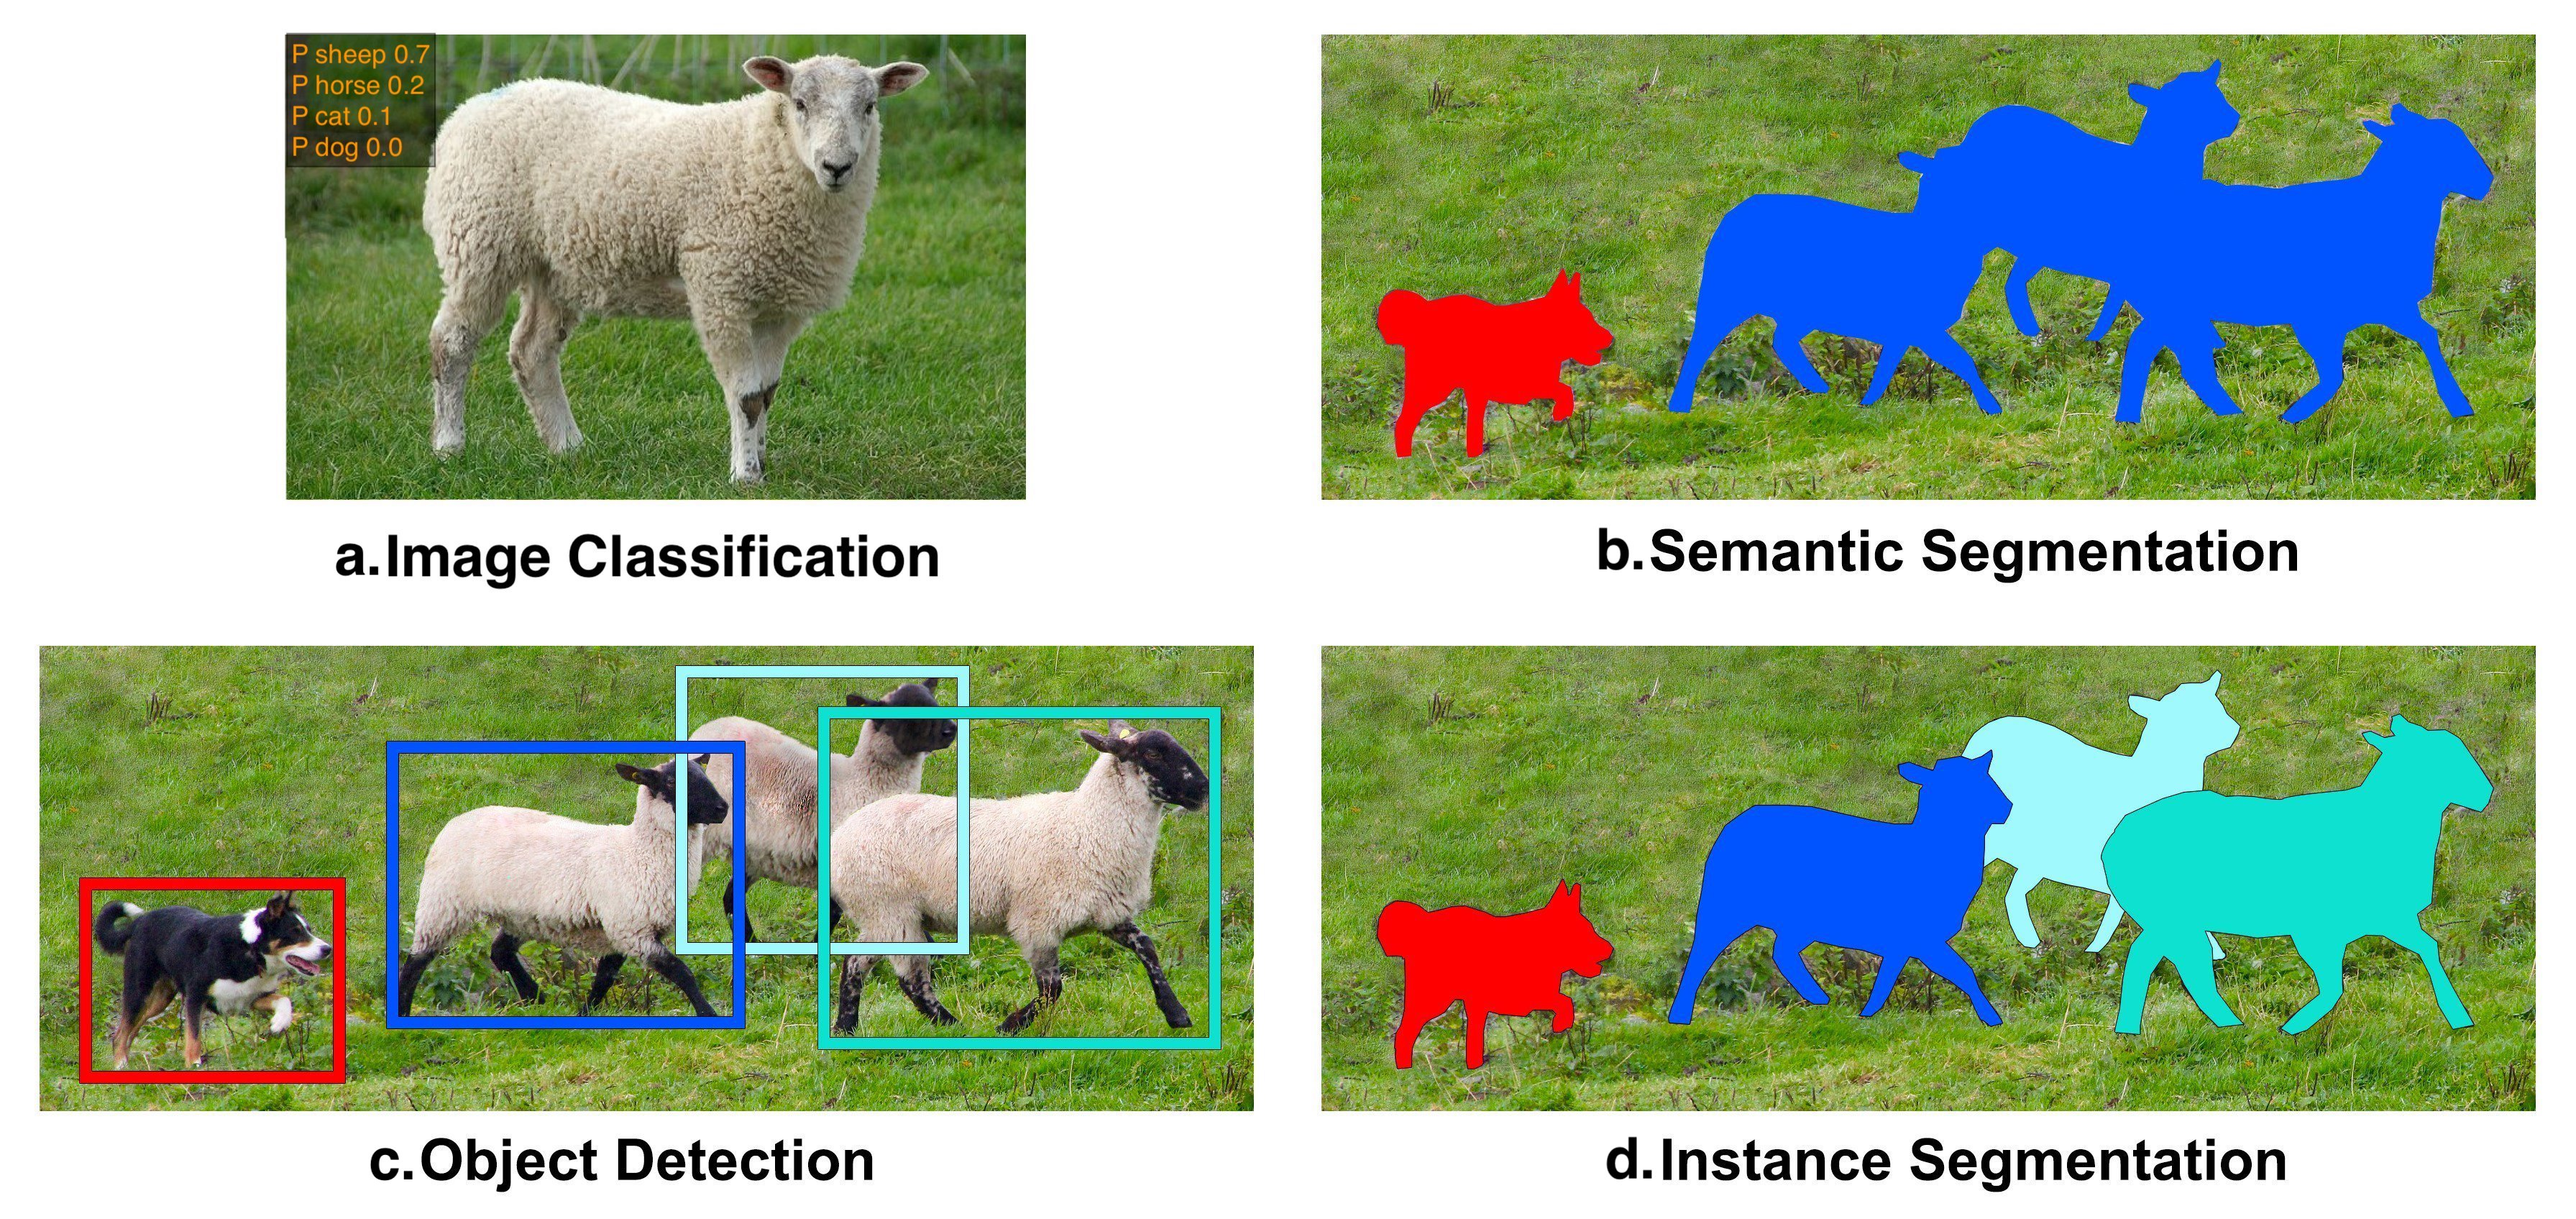
\includegraphics[width=4in]{figures/diff_cv_tasks.jpeg}
    \caption{Different Computer Vision Tasks \cite{diff_detection_segmentation_task_fig}}
    \label{fig:diff_cv_tasks}
\end{figure}

We begin with image classification, the most fundamental task in the computer vision field. The task involves assigning an object category label to an input image, assuming the input image contains exactly one object \cite{overview_cv_task}. This implies that the task allows the object classification label to be given to the entire image without specifying where the object is. As shown in Figure \ref{fig:diff_cv_tasks}a, the image classification model predicts the probability that the image shows a sheep, a horse, a cat, or a dog. Although image classification is comparatively simpler than other computer vision tasks, it presents several significant challenges due to the variability of image appearance caused by changes in scale, orientation, lighting, occlusions, and other factors.

The second task is semantic segmentation. In contrast to image classification, semantic segmentation is unconcerned with the presence or absence of objects in the input image. The objective of the task is to classify each pixel of the input image into one of several predefined classes or categories \cite{overview_cv_task}. By classifying each pixel, the task generates a detailed mapping between image pixels and classes that can be used to locate and outline objects of different classes within the image. However, when classifying each pixel without consideration of object location, the task removes the depth dimension of the image. That is, if two objects of the same class are positioned behind one another, then the semantic segmentation model will consider them as one object of this class, thus losing dimension information. Considering Figure \ref{fig:diff_cv_tasks}b, we noted the three sheep are at different locations in the depth dimension, but the semantic segmentation mask visualizes these sheep as one object in 2-dimensional space.

The third task is object detection, an improvement over image classification. The goal of object detection models is to locate and categorize each object within a given image \cite{overview_cv_task}. The process of object detection involves two main subtasks: object localization and object classification. Object localization determines the location and size of each object in an image by predicting a bounding box around the object. Once the object is localized, it can be classified using an image classification model. Compared to semantic segmentation, object detection retains all spatial information of the object in the image but loses the pixel accuracy mask. This is illustrated in Figures \ref{fig:diff_cv_tasks}c and \ref{fig:diff_cv_tasks}d, where object detection is able to detect all three sheep, but it is unclear whether a pixel within the bounding box refers to the sheep or the grass behind it.

The last task we want to discuss is instance segmentation. For every object in a given image or video frame, the instance segmentation model must identify all pixels belonging to the object and assign a category label to the object \cite{overview_cv_task}. Identifying all pixels that belong to the object creates the object's mask, which may then be used to locate pixel-precise locations and the object's outline. While object detection and instance segmentation involve locating objects, the former offers information about the location and scale of the detected objects, whereas the latter goes further by identifying all pixels associated with the object. On the other hand, the main distinction between instance and semantic segmentation lies in the level of detail they provide. While semantic segmentation divides an image into classes such as "vehicle" or "animal", instance segmentation provides more details by distinguishing between each individual object within those classes. It accomplishes this by assigning each object a unique label for identification. This means that instance segmentation can determine not only the class of each object in an image but also where it is located and how many there are - something semantic segmentation cannot achieve on its own. Considering Figure \ref{fig:diff_cv_tasks}, we observed that instance segmentation creates a pixel-accurate outline of all four animals, in contrast to the bounding box generated by object detection. In addition, the instance segmentation model's pixel-by-pixel mask must differentiate between the three sheep in contrast to semantic segmentation. In other words, the instance segmentation model combines object detection and semantic segmentation strengths while eliminating their weaknesses.
 
R-CNN and YOLO are two popular families of models used for object detection and instance segmentation. In Chapters \ref{chap:rcnn_variation} and \ref{chap:yolo_variation}, we will delve into the variations of R-CNN and YOLO model, respectively. However, before we proceed, it is essential to understand the metrics used for assessing the performance of an object detection or instance segmentation model. In the next subsection, we will discuss the metrics utilized for evaluating these models.